\documentclass[aspectratio=169]{beamer}

\usepackage{booktabs}
\usetheme{default}
\setbeamertemplate{navigation symbols}{}
\setbeamertemplate{itemize item}{\color{black}\textbullet}
\setbeamertemplate{itemize subitem}{\color{black}\textbullet}
\usepackage{xcolor}
\usepackage{tikz}
\usetikzlibrary{shapes,positioning,arrows}
\definecolor{navy}{RGB}{0, 0, 128}
\definecolor{lightblue}{RGB}{173, 216, 230}
\definecolor{lightgreen}{RGB}{144, 238, 144}
\definecolor{lighterlightblue}{RGB}{230, 245, 255}
\definecolor{lighterlightgreen}{RGB}{240, 255, 240}
\newcommand{\highlight}[1]{\colorbox{lightblue}{$\displaystyle\textcolor{navy}{#1}$}}
\newcommand{\highlighttext}[1]{\colorbox{lightblue}{\textcolor{navy}{#1}}}


\begin{document}

\begin{frame}
\textcolor{navy}{Bellman Equation} for dynamic discrete choice:
\begin{align*}
V_{it} &= \mathbb{E}\max_{j \in \mathcal{J}}\left\{u_{ijt} + \beta V_{it+1}(X_{it+1}) + \epsilon_{ijt}\right\}
\end{align*}
\end{frame}



\begin{frame}
Estimation algorithm:
\bigskip{}

\begin{enumerate}
\itemsep1.5em
    \item<2-> Start with initial guess of $(\alpha,\beta,\gamma)$
    \item<3-> Solve value functions $v_{jt}$ backwards from terminal period using Bellman equation
    \item<4-> Compute policy functions (choice probabilities, $p_{jt}(X_{it};\alpha,\beta,\gamma)$) using current $v_{jt}$'s
    \item<5-> Evaluate log likelihood $\ell(\alpha,\beta,\gamma)$ and update parameter guesses
    \item<6-> Repeat steps 2--5 until convergence
\end{enumerate}

\end{frame}



\begin{frame}

\begin{columns}[T]
\column{0.48\textwidth}
\centering
\textcolor{navy}{\hspace{1cm}Traditional Approach}
\bigskip{}

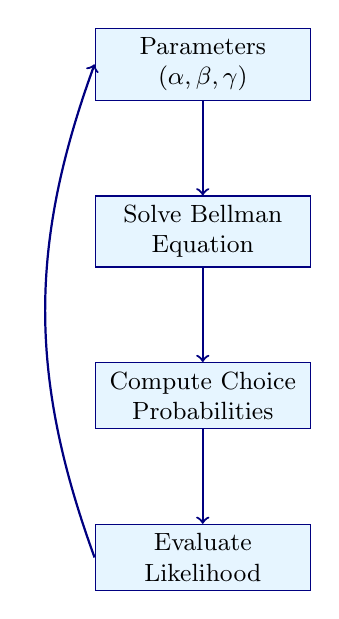
\begin{tikzpicture}[
    box/.style={rectangle, draw=navy, fill=lighterlightblue, text width=2.5cm, text centered, minimum height=0.8cm, font=\small},
    arrow/.style={->, navy, thick},
    node distance=1.2cm
]

\node[box] (params) {Parameters\\$(\alpha,\beta,\gamma)$};
\node[box, below=of params] (solve) {Solve Bellman\\Equation};
\node[box, below=of solve] (policy) {Compute Choice\\Probabilities};
\node[box, below=of policy] (likelihood) {Evaluate\\Likelihood};

\draw[arrow] (params) -- (solve);
\draw[arrow] (solve) -- (policy);
\draw[arrow] (policy) -- (likelihood);
\draw[arrow] (likelihood.west) to [bend left=20] (params.west);

\end{tikzpicture}

\column{0.48\textwidth}
\centering
\textcolor{navy}{CCP Approach}
\bigskip{}

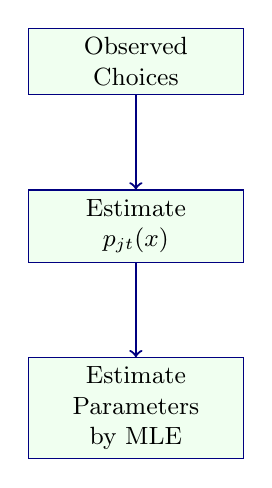
\begin{tikzpicture}[
    box/.style={rectangle, draw=navy, fill=lighterlightgreen, text width=2.5cm, text centered, minimum height=0.8cm, font=\small},
    arrow/.style={->, navy, thick},
    node distance=1.2cm
]

\node[box] (data) {Observed\\Choices};
\node[box, below=of data] (ccps) {Estimate\\$p_{jt}(x)$};
\node[box, below=of ccps] (extract) {Estimate\\Parameters\\by MLE};

\draw[arrow] (data) -- (ccps);
\draw[arrow] (ccps) -- (extract);

\end{tikzpicture}

\end{columns}

\vspace{1cm}
\begin{center}
\large\textcolor{navy}{\textbf{Key Insight:} Extract structure from choice patterns, not value functions}
\end{center}

\end{frame}

\begin{frame}
    $$\log\left(\frac{p_{1t+1}}{p_{0t+1}}\right) = v_{1t+1} - v_{0t+1}$$
\end{frame}


\begin{frame}
\textcolor{navy}{Example:} Bus maintenance decisions

\bigskip

\begin{columns}[T]
\column{0.48\textwidth}
\begin{center}
Raw Data\bigskip\par
\begin{tabular}{cc}
\toprule
Mileage & Choice \\
\midrule
50,000 & Keep \\
75,000 & Keep \\
120,000 & Replace \\
140,000 & Replace \\
\vdots & \vdots \\
\bottomrule
\end{tabular}
\end{center}

\column{0.48\textwidth}
\begin{center}
Choice Probabilities\bigskip\par
\begin{tabular}{cc}
\toprule
Mileage & $P(\text{Replace})$ \\
\midrule
50,000 & 0.05 \\
75,000 & 0.15 \\
100,000 & 0.45 \\
125,000 & 0.80 \\
150,000 & 0.95 \\
\bottomrule
\end{tabular}
\end{center}
\end{columns}

\vspace{0.5cm}
\textcolor{navy}{No structural assumptions needed yet!}

\end{frame}

\begin{frame}
\only<1>{
$$V_{t+1} = v_{jt+1} - \ln p_{jt+1} + c$$
}
\only<2>{
$$V_{t+1} = \highlight{v_{jt+1}} - \ln p_{jt+1} + c$$
}
\only<3>{
$$V_{t+1} = \highlight{v_{jt+1}} - \ln p_{jt+1} + c$$
\bigskip\par
$$\highlight{v_{jt+1}} = u_{jt+1} + \beta \mathbb{E}\left[V_{t+2}\vert d_{t+1}=j\right]$$
}
\end{frame}

\end{document}